\documentclass{article}

    % Input language encoding
    %\usepackage[utf8]{inputenc}
   
    % Output languages
    %\usepackage[greek, english]{babel}
    % \usepackage{alphabeta}
    
    % Fonts
    %\usepackage[T1,LGR]{fontenc}
    \usepackage{lmodern}

    % Images
    \usepackage{graphicx}
    \graphicspath{ {./images/} }
    \usepackage{float}
    \usepackage{caption}
    \usepackage{subcaption}

    % Math
    \usepackage{amsmath}

    % Paragraph Formatting
    \usepackage{parskip}

    % Code
    \usepackage{listings}
    \usepackage{clrscode3e}


    % Computer Array Drawings
    \usepackage{tikz}
    \usetikzlibrary{calc}
 

        

    \DeclareMathSizes{10}{10}{10}{10}
    \setlength{\parindent}{0cm}

    \title{Chapter 2 Part 1 Exercises}

\begin{document}

\pagenumbering{gobble}
\date{}
\author{}

\maketitle

\section*{2.1-1}

The steps are the following:

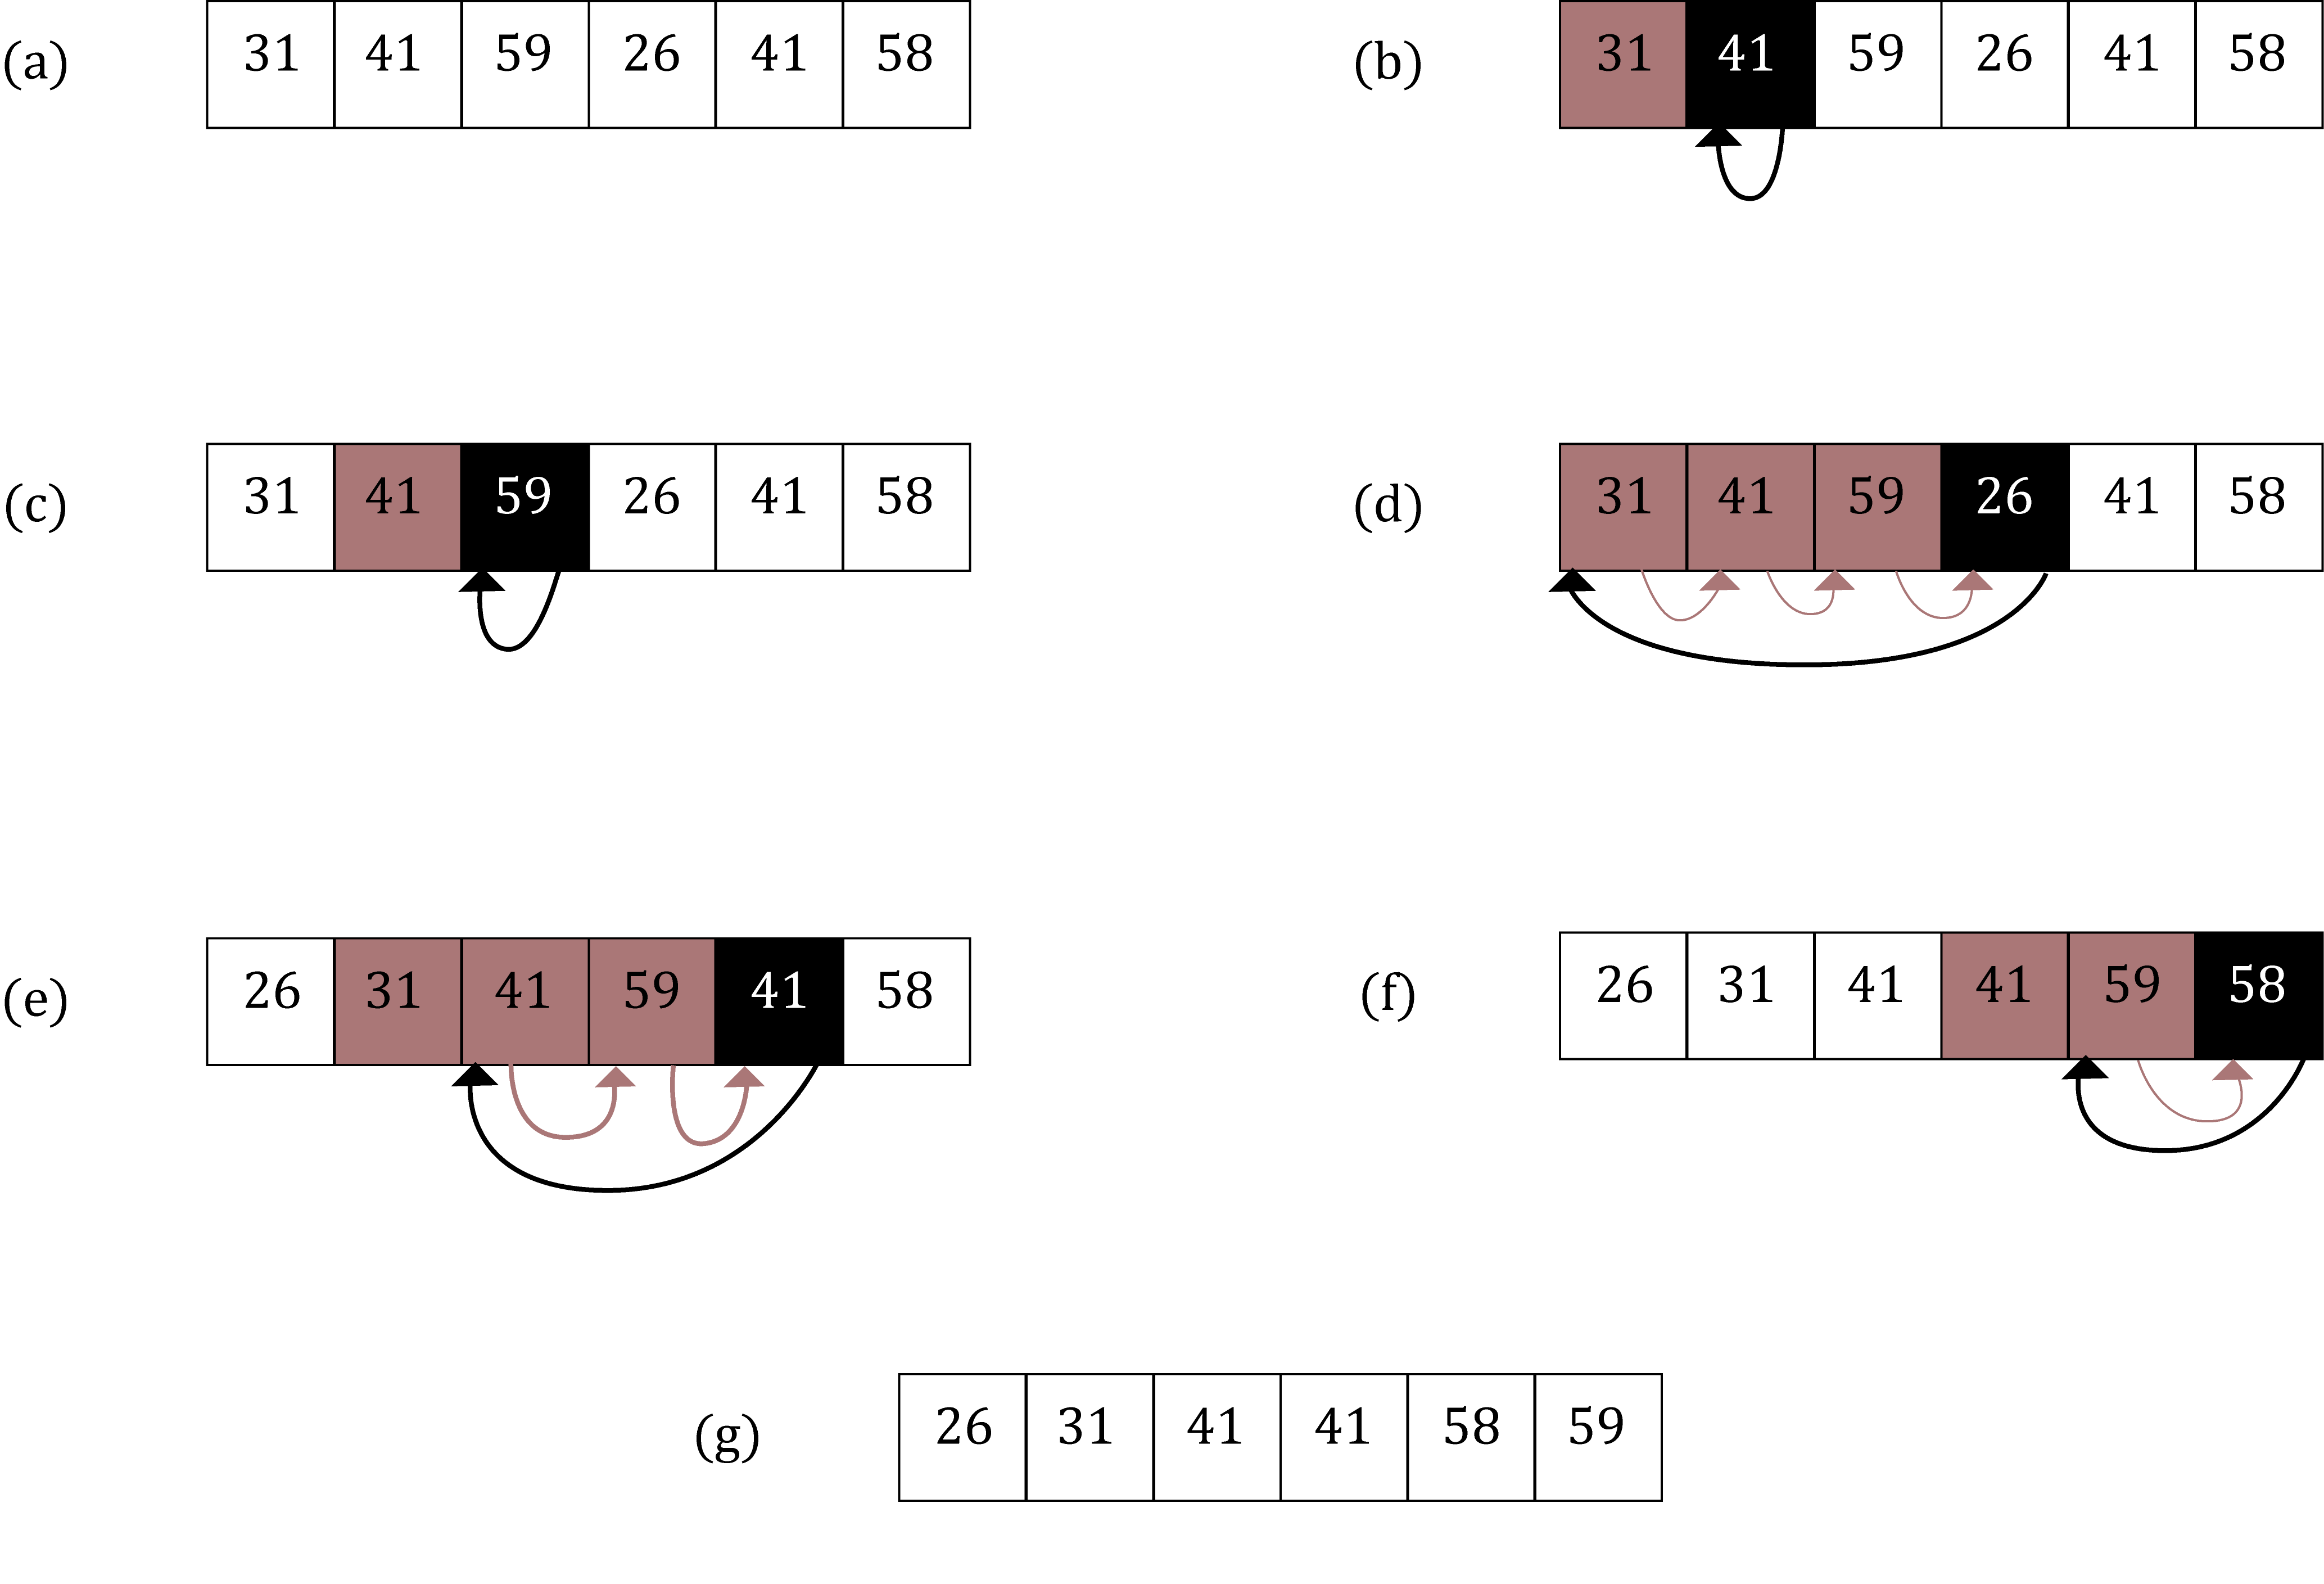
\includegraphics[scale=0.3]{2_1-1.png}

\section*{2.1-2}

The new instertion-sort will be the following:

\begin{codebox}
    \Procname{$\proc{Reverse-Insertion-Sort}(A)$}
    \li \For $j \gets 2$ \To $\attrib{A}{lenght}$
    \li   \Do            
          $\id{key} \gets A[j]$
    \li   $i \gets j-1$
    \li   \While $i > 0$ and $A[i] < \id{key}$
    \li     \Do
            $A[i+1] \gets A[i]$
    \li     $i \gets i-1$
            \End
    \li   $A[i+1] \gets\id{key}$
          \End
\end{codebox}

\section*{2.1-3}

The linear search algorithm will be:

\begin{codebox}
  \Procname{$\proc{Linear-Search}(A, v)$}
  \li \While $i \leq \attrib{A}{length}$
  \li \Do
        \If $A[i] \isequal v$
  \li   \Then
          \Return $i$
        \End
  \li     $i \gets i + 1$
      \End
  \li \Return \const{nil}
\end{codebox}

If the linear search finishes, then $v$ has not been found in the array, so we return NIL. Otherwise, the loop stops when the first occurance of $v$ is found.

The \textbf{loop invariant} of the algorithm is: 

\begin{center} \textit{
  At the start of each iteration of the loop, the subarray $A[1..i-1]$ does not hold the value $v$. }
\end{center}

Let us see now how the loop invariant properties hold now.

\textbf{Initialization:} We start by showing that the loop invariant holds before the first loop operation, when $i = 1$. The subarray of A is empty, so by definition it does not contain v. 

\textbf{Maintenance:} Informally, the body of the while loop compares $v$ with $A[i]$ and exits the loop if they are equal. The subarray $A[1..i]$ consists of elements that are not equal to $v$, as otherwise the loop would have ended.

\textbf{Termination:} We examine what happens when the loop terminates. When the loop terminates the value of $i = A.lenght + 1 = n + 1$. Then, the whole array $A$ is the left subaray $A[1...i]$, so we have gone through the whole array and not found the value $v$, so we return NIL.

\section*{2.1-4}

Stating the problem formally:

\textbf{Input:} Two arrays A, B of size n containing binary digits.

\textbf{Output:} An array C, which is of size $n+1$ and contains the binary sum of A and B.

\textbf{Code:}

\begin{codebox}
  \Procname{$\proc{Binary-Addition}(A, B, C)$}
  \li $\id{carry} = 0$ 
  \li \For $i \gets$ \attrib{A}{length} \Downto $1$
  \li \Do
        $C[i+1] \gets A[i] + B[i] + \id{carry}$
  \li   \If $C[i+1] \isequal 2$ 
  \li   \Then
          $C[i+1] \gets 0$
  \li     $\id{carry} \gets 1$
  \li   \ElseIf $C[i+1] \isequal 3$  
  \li   \Then
          $C[i+1] \gets 1$
  \li     $\id{carry} \gets 1$
  \li   \Else
  \li     $\id{carry} \gets 0$
        \End
      \End
  \li $C[1] \gets carry$
\end{codebox}


\end{document}